

\section{Association Analysis}
\subsection{Introduction(*)}

L'analisi di associazione ci riporta al concetto di causalit\`a di variabili: dati certi valori di attributi cosa posso dire del valore di un altro attributo?

Le regole associative ci permettono di prendere delle scelte molto operative in diversi ambiti, in particolare in quello che viene chiamato \textit{market busket analysis}. 
Il problema del carrello tratta il posizionamento di prodotti in un negozio. Si sa che all'acquisto di un certo prodotto si tende a acquistare altri prodotti connessi, quindi si cercano queste associazioni basandosi sul carrello della spesa dei clienti (appunto market basket) per poi capire come impostare la disposizione sugli scaffali.

\textbf{Obiettivo}: identificare quali siano gli \textbf{item associati} per poter prendere delle decisioni. In sostanza si generano \textbf{Regole associative} formate da coppie di insiemi \textit{antecedente} e \textit{conseguente}.

es. \{Beer\} $\rightarrow$ \{swiss cheese\} 

\quad \{antecedente\} $\rightarrow$ \{conseguente\}\\
\textbf{NB}: non \`e una causalit\`a ma un'associazione

L'analisi si basa sullo studio di due diversi dataset:
\begin{itemize}
	\item Product set: contiene informazioni legate ai prodotti come il nome e il prezzo
	\item Transaction set: contiene informazioni legate agli acquisti dei clienti, ogni record corrisponde ai prodotti presenti nel carrello del cliente
\end{itemize}

Si organizza il dataset delle transazioni in formato binario, ovvero ogni colonna indica se in una data transazione un certo prodotto sia o meno presente.

\begin{figure}[H]
	\centering
	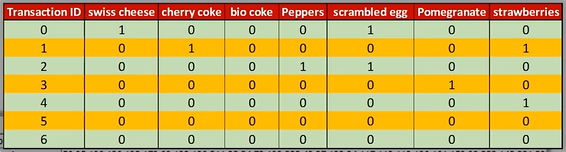
\includegraphics[height=0.25 \linewidth]{association/pict/transaction_set_bin.png}
	\caption{esempio: transaction set binarizzato}
\end{figure}
\clearpage
\noindent
Consideriamo:

$I = \{i_1, i_2,...,i_d\}$ il set di tutti gli item nel market basket

$T = \{t_1,t_2,...,t_N\}$ l'insieme di tutte le transazioni

\begin{defn}
	Una collezione di zero o più item è chiamata \textbf{Itemset}.
\end{defn} 
\begin{defn}
	Se un itemset contiene k item \`e detto \textbf{K-Itemset}.
\end{defn}
\begin{defn}
	L'itemset che non contiene alcun elemento è detto \textbf{empty set}.
\end{defn}
\begin{defn}
	La \textbf{transaction width} è il numero di item presenti in una transazione
\end{defn}
	 
Una transazione $t_j$ contiene l'itemset $X$, se $X$ è un sottoinsieme di $t_j$.
RIPRENDERE QUAAAAAAAAAAAAAAAAAAAAAAAAAAAAAAAAAAAAAAAAAAAAAAAAAAAAAA
Per comprendere la frequenza degli item in una transazione si considera il \textbf{Support count}. Un itemset viene valutato anche dal numero di transazioni che lo contengono, conteggiato nel $Support Count$:

\[ \sigma(X) = |\{t_i | X  t_i, t_i \in T\} \] SBAGLIATA

Una \textbf{regola di associazione} viene rappresentata come:

$X \rightarrow Y$

dove X e Y sono itemset disgiunti ($X \cap Y = \emptyset$), una regola viene valutata in termini di supporto e confidenza.

\textbf{Support} determina quanto spesso una regola sia applicabile dato un data set:

\[s\{x \rightarrow Y\} = \frac{\sigma(X \cup Y)}{N}\]

\textbf{Confidence} determina quanto frequente Y \`e presente in una transazione che contiene X (si assume che l'universo sia rappresentato partendo da X):

\[c\{x \rightarrow Y\} = \frac{\sigma(X \cup Y)}{\sigma(X)}\]

Perch\`e utiliziamo il supporto:
\begin{itemize}
	\item potrebbe esserci un'associazione casuale se troppo basso
	\item potrebbe non valere la pena seguire associazioni che si applicano in modo poco significativo dal punto di vista dei profitti 
\end{itemize}
Supporto utilizzato per eliminare regole non desiderate e condivide interessanti propriet\`a che possono essere sfruttate per la ricerca di regole associative efficaci.

La confidenza \`e molto importante perch\`e un alta confidenza significa che Y sar\`a molto presente in transazioni con C e si stima la probabilit\`a  condizionata di Y dato X.

\textbf{Association Rule Mining Problem}:

dato un set di transazioni T, trovare le regole con support $\ge$ minsup e confidence $\ge$ minconf.

Approccio a forza bruta di association rule non \`e molto praticabile in quanto i tempi di computazione aumentano in modo esponenziale: $R = 3^d - 2^{d+1} + 1$.

Una strategia comunemente adottata in molti algoritmi \`e decomporre il problema in 2 grandi supertask:
VEDI CHRISTIAN


\subsection{Generazione di frequent itemset e generazione regole}

Un itemset \`e frequente se supera la soglia fissata di minima frequenza per essere considerato tale. 
\textbf{Candidate Itemset}: ovvero l'insieme di tutti gli itemset che possiamo formare. Avranno un numero di item diverso. 

Se procediamo con un approccio forza bruta per trovare gli \textbf{itemset frequenti} bisogna determinare il support count per ogni itemset candidato. \\
I confronti da effettuare sono nell'ordine di O(NMw), dove N = numero di transazioni, M = numero di itemset candidati e w = massima lunghezza delle transazioni. 

\`E troppo come numeri confronti contando che molti dei quali sono inutili o poco significativi.

Vi sono due approcci per ridurre il costo computazionale della generazione di itemset frequenti:
\begin{itemize}
	\item ridurre il numero di candidati itemset. Il principio Apriori \`e un metodo per eliminare alcuni candidati itemset senza contare il support count. Principio: se un itemset \`e frequente, allora tutti i suoi sottoinsiemi sono frequenti
	\item riduce il numero di confronti anzich\`e controllare tutte le possibili combinazioni, lo si fa con strutture dati avanzate
\end{itemize}

Il principio apriori si basa sul fatto che se una regola ha una frequenza bassa allora tutte le regole che prevedono come sottoinsieme la stessa non supereranno quella frequenza pertanto \`e inutile considerarle. Posso quindi fare \textbf{pruning} dell'albero per queste soluzioni, viene chiamato \textbf{support-based pruning}.

\subsection{Algoritmo apriori}
Genera due operazioni:
\begin{itemize}
	\item Candidate Generation: genera nuvi candidati k-itemset basati su (k-1)-itemset frequenti calcolati nella precedente iterazione
	\item Candidate Pruning: questa operazione elimina alcuni candidati k-itemset usando la strategia del support-based pruning
\end{itemize}

La complessit\`a computazionale soffre di 4 limiti:
\begin{itemize}
	\item Support threshold: la soglia di supporto se troppo bassa non taglio molto l'albero, per\`o non deve essere neanche troppo elevata. 
	\item Numero di item (dimensionalit\`a): se il numero di item cresce, pi\`u spazio ci sar\`a bisogno in memoria per registrare il support count degli item.
	\item numero di transazioni: e molto grande bisogna scorrere ogni volta tutta la lista
	\item avarage transaction width: quanto \`e mediamente densa la lista di item. La massima taglia di itemset frequenti tende ad aumentare la width delle transazioni media,
\end{itemize}

\subsection{Rule Generation}
Ogni k-itemset frequente, Y pu\`o generare al limite $2^k-2$ regole di associazione. 

Una regola di associazione pu\`o essere estratta partizionando itemset Y in 2 sottoinsiemi non vuoti: $X \rightarrow Y -X$ che soddisfa il threshold di confidenza.

Tutte le regole generate da itemset frequenti sono esse stesse frequenti.

In pratica, il numero di itemset frequenti prodotti da transazioni possono essre molto grandi. Per questo si ragiona in due rappresentazioni:
\begin{itemize}
	\item Maximal Frequent Itemset
	\item closed Frequent Itemset
\end{itemize}

\textbf{Maximal Frequent Itemset}: verifica il vincolo della frequenza e definisce la frontiera dove lui non gode pi\`u di questa propriet\`a, massima frontiera in cui mi posso spingere. Lo \`e se lui \`e frequente e se tutte le sue estensioni non sono frequenti.\\
Fornisce una rappresentazione compatta dell'insieme di itemset che cerchiamo, la pi\`u piccola espressione in cui gli itemset sono derivabili. Il maximal frequent itemset \`e applicabile solo se si utilizzano algoritmi efficienti che cerca tutti e solo gli itemset massimali.

Per costruzione per\`o non ci dice quanto \`e la sua confidenza rispetto ai suoi sottoinsiemi. 

\textbf{Closed Frequent Itemset}: un itemset X \`e chiuso se nessun immediato sottinisme ha esattamente lo stesso support count di X. In ogni caso il suo spporto deve essere maggiore o uguale a minsup.

Importante qunado vi sono gruppi di prodotti venduti a blocco ignorando gli altri.

Questo tipo di itemset sono utili per rimuovere regole di associazione ridondanti. 

Una regola di associazione $X \rightarrow Y$ \`e ridondante se esiste $X' \rightarrow Y'$ che rispetta certe propriet\`a. (vedi Christian)

\begin{figure}[H]
	\centering
	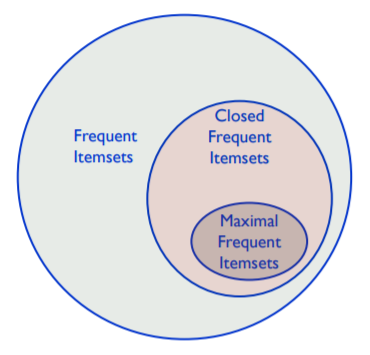
\includegraphics[height=0.45 \linewidth]{association/pict/itemset_freq.png}
	\caption{gerarchia dei frequent itemset}
\end{figure}

